\documentclass{article}

% if you need to pass options to natbib, use, e.g.:
%     \PassOptionsToPackage{numbers, compress}{natbib}
% before loading neurips_2018

% ready for submission
% \usepackage{neurips_2018}

% to compile a preprint version, e.g., for submission to arXiv, add add the
% [preprint] option:
%     \usepackage[preprint]{neurips_2018}

% to compile a camera-ready version, add the [final] option, e.g.:
\usepackage[final]{nips_2018}

% to avoid loading the natbib package, add option nonatbib:
%     \usepackage[nonatbib]{neurips_2018}

\usepackage[utf8]{inputenc} % allow utf-8 input
\usepackage[T1]{fontenc}    % use 8-bit T1 fonts
\usepackage{hyperref}       % hyperlinks
\usepackage{url}            % simple URL typesetting
\usepackage{booktabs}       % professional-quality tables
\usepackage{amsfonts}       % blackboard math symbols
\usepackage{nicefrac}       % compact symbols for 1/2, etc.
\usepackage{microtype}      % microtypography
\usepackage{graphicx}
\usepackage{subcaption}
\usepackage{amsmath}
\usepackage{multirow} 


\graphicspath{ {imgs/} }

\title{Repo Velocity: Diagnosing Git Repository Health}

% The \author macro works with any number of authors. There are two commands
% used to separate the names and addresses of multiple authors: \And and \AND.
%
% Using \And between authors leaves it to LaTeX to determine where to break the
% lines. Using \AND forces a line break at that point. So, if LaTeX puts 3 of 4
% authors names on the first line, and the last on the second line, try using
% \AND instead of \And before the third author name.

\author{%
  Tyler Brown\\
  \texttt{NUID: 001684955} \\
  % Coauthor \\
  % Affiliation \\
  % Address \\
  % \texttt{email} \\
  % \AND
  % Coauthor \\
  % Affiliation \\
  % Address \\
  % \texttt{email} \\
  % \And
  % Coauthor \\
  % Affiliation \\
  % Address \\
  % \texttt{email} \\
  % \And
  % Coauthor \\
  % Affiliation \\
  % Address \\
  % \texttt{email} \\
}

\begin{document}
% \nipsfinalcopy is no longer used

\maketitle

\section{Introduction}

Understanding the health of open source projects is important to
industry because it helps them assess risk associated with their
technology stack. Forecasting health is important to investors because
this information can help them make profitable investments in open
source. Academia is interested to know if there are links between
theory, such as programming language design \cite{ray2014large}, and the
health of open source software. A previous metric used to assess open source
software health is the Truck Factor \cite{avelino2015truck}. Truck Factor
is the smallest subset size of developers who contributed 50\% of the code
in an open source project. The underlying intuition is that open source
projects with a lower Truck Factor are more susceptible to project disruption
in the event of adverse circumstances.

By borrowing from Physics, this paper
\footnote{Code available on GitHub: https://github.com/tbonza/EDS19}
contributes to the advancement of understanding the health of open source
projects, studying a subset of GitHub repositories, with the following:

\begin{itemize}
\item Introducing a health measure that can be assessed at time
  $t_{i \pm k}$ where $k$ is a multiple of $i$.
\item New health measure can be used in forecasting as well as description
\item Health measure is rooted in Physics so we can derive related measures
  using preexisting theory.
\end{itemize}

\section{Related Work}

Truck Factor reflects robustness of project \cite{avelino2015truck} by
computing the minimum number of developers required to comprise 50\% of
file ownership. The underlying intuition is that a project with a low
number of dominant developers will be more susceptible to failing due
to external shocks. Projects where file ownership is shared by a large
number of developers are interpreted as more healthy with this approach.

Not all projects reflects software which requires support. Researchers have
classified many project types such as 'software development projects',
'solutions for homework', 'projects with educational purposes', 'data sets',
and 'personal web sites' \cite{soll2017classifyhub}. The observation that
many projects are not software development is also a noted peril when
analyzing GitHub \cite{kalliamvakou2016depth}. We may also find repositories
containing code duplicates \cite{lopes2017dejavu}. These factors may
comprise threats to validity which are important to address in this analysis.

\section{Methods}

The Truck Factor assesses Git repository health at time $t_i$. We would
like to better understand health at different points in time $t_{i \pm k}$
where $k \ge 1$. We can borrow from Physics to find such a measure. Velocity,
$v(t)$, is a measure of distance over time. What is a proxy for distance in
the context of Git repository health? Total lines of code changed in a
project during time $t_i$ can tell us how quickly the code base is
changing. We apply this definition of velocity, $v(t)$, for our new measure
Repo Velocity.

\begin{equation} \label{eq:1}
  \text{Repo Velocity } \approx v(t) = \frac{d}{t} =
  \frac{\text{lines added } - \text{ lines deleted}}{t}
  \qquad \forall i \pm k \in t | i \in \mathbb{R}, k \in \mathbb{R}_{>0}
\end{equation}

Equation \ref{eq:1} defines our target measure, Repo Velocity, and posits
that the Physics concept of 'distance' can provide insight into how a GitHub
repository is changing over time. We can compute velocity, $v(t_i)$ at time
$t_i$ where $i$ is a real number. We can also compute average velocity,
$v_{avg}(t_{i \pm k})$, at time $t_i$ to time $t_{i \pm k}$. The Repo
Velocity measure also has the advantage of allowing aggregation and
disaggregation. Truck Factor is a measure which can only be analyzed at an
aggregate level. There can be a lot of interesting variation below a
Repository level aggregation. Repo Velocity can also be used to capture
individual contributor velocity. The ability of Repo Velocity to be applied
over time as well as at aggregated and disaggregated levels make the measure
a unique contribution to the understanding of Git repository health. The
remaining methodology seeks to establish Repo Velocity as an informative
descriptive and predictive target or dependent variable.

\subsection{Establishing Baseline Repo Velocity}

In our effort to establish the Repo Velocity measure, we first examine
behavior on Git repositories known to be either (a) active and currently
in development, (b) previously active and not currently in development. The
repositories I chose for the baseline subset are as follows:

\begin{enumerate}
\item torvalds/linux (a) - Linux kernel, a fundamental component in many
  cloud computing server operating systems such as Amazon Linux.
\item docker/docker-ce (a) - Community edition of Docker including the open
  repositories Docker Engine and Docker client, a popular enterprise
  application container platform currently heavily utilized in projects
  such as Kubernetes.
\item apache/spark (a) - Unified analytics engine for Big Data. Allows for
  an alternative to Map/Reduce and is currently widely favored by industry.
  One of the most active projects in the Apache Software Foundation
  \cite{TheApach51:online}.
\item apache/lucene-solr (a) - Mirror of Apache Lucene + Solr. Apache Lucene
  is a high-performance, full featured text search engine library written in
  Java. Apache Solr is an enterprise search platform written using Apache
  Lucene. Notably, Lucene is a major dependency for Elasticsearch
  \cite{elastics3:online}
\item apache/attic-lucy (b) - Mirror of Apache Lucy, search engine library
  provides full-text search for dynamic programming languages. Previously
  active project in the Apache ``attic''.
\item apache/attic-wink (b) - Apache Wink, simple yet solid framework for
  building RESTful Web services. Previously active project in the Apache
  ``attic''.
\end{enumerate}

All GitHub repositories chosen for the baseline sample would be classified
as 'software development projects', or \textit{DEV}\footnote{The baseline
  distribution containing only DEV repositories is a fundamental part of
  the results presented in this paper.} using the ClassifyHub designations
\cite{soll2017classifyhub}. This paper establishes baseline Repo Velocity
expectations using descriptive and predictive (forecasting) methodologies.

\subsubsection{Descriptive Baseline}

We establish a descriptive baseline for the Repo Velocity measure by
examining changes the measure over time (2013-2018) across our baseline
sample. Figure \ref{fig:desc_baseline} shows diverging behavior within the
baseline sample for repositories which are (a) active and currently in
development, or (b) previously active and not currently in development. The
common trend with (b) type repositories is that Repo Velocity is converging
to zero. Apache Lucy (b), shows a decrease in velocity then a convergence to
zero between 2013 and 2015. Apache Wink (b) has already converged to zero
within the 2013-2018 time window; a longer term window shows similar
behavior to Apache Lucy.

\begin{figure}[h]
  \centering
  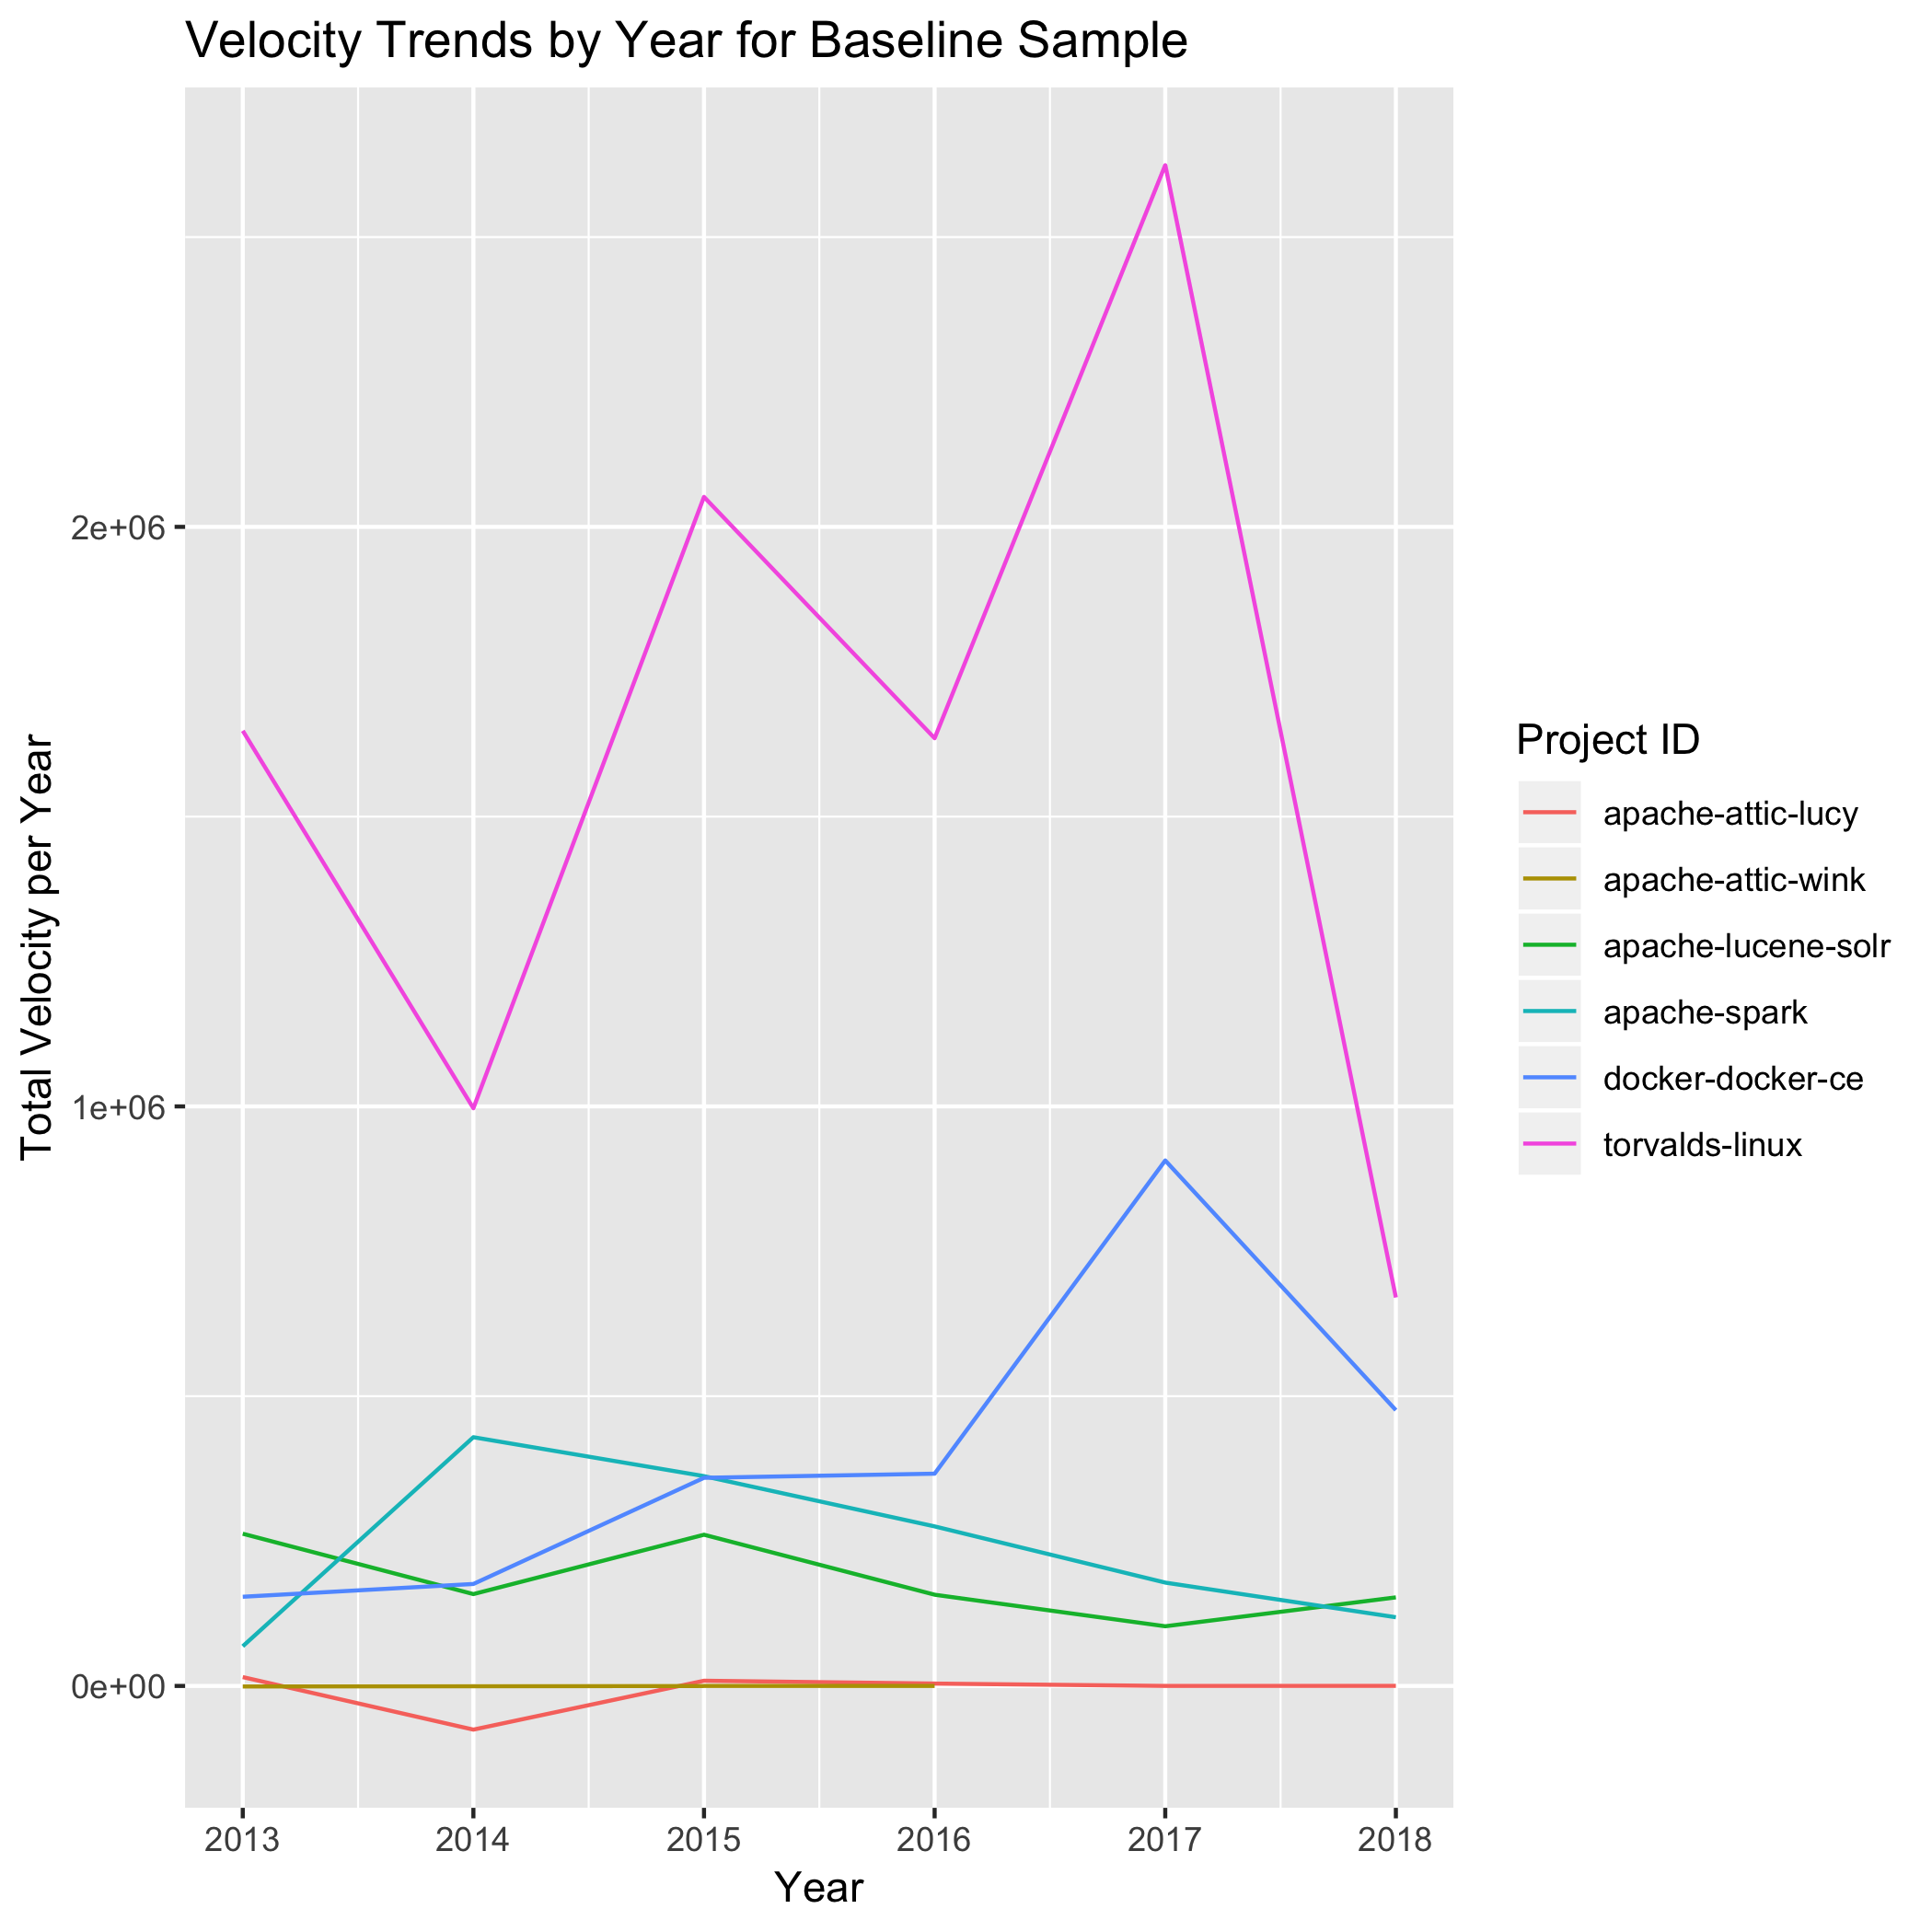
\includegraphics[scale=0.15]{f3}
  \caption{Repo Velocity Trends for Baseline Sample}
  \label{fig:desc_baseline}
\end{figure}

Type (a) projects show considerable variance in Repo Velocity, such as
'torvalds/linux'. However, on average, we can see that Repo Velocity is
not converging to zero. There is a clear and interesting trend with Apache
Spark that is showing a downward trend in Repo Velocity between 2014 and
the end of sample at December 2018. This downward trend may reflect a peril
of mining GitHub \cite{kalliamvakou2016depth}, in that not all repositories
are projects. For example, Yahoo is currently developing
TensorFlowOnSpark \cite{yahooTen24:online} which allows Tensorflow
programs to operate using Apache Spark clusters. The Yahoo project is
directly competing with an offering by Google Cloud which does not appear
to involve Spark \cite{RunningD43:online}. We can see that GitHub
repositories not representing the scope of a project is a potential
threat to validity we must consider here.

Trends viewed in this descriptive baseline helped to inform the following
hypothesis:

\begin{itemize}
\item[$H1_{a}$]: As the absolute value of velocity diverging from zero
  (acceleration) increases, Git repo health will also increase.
\end{itemize}

Hypothesis $H1_{a}$ should hold when reviewing the predictive baseline,
as well as at scale.

\subsubsection{Predictive Baseline}

The predictive baseline uses Repo Velocity as a target or dependent variable
and seeks to explain which features contribute to this measure. This paper
posits the following features play a strong role in explaining Repo Velocity:

\begin{itemize}
\item Number of authors in a given time period.
\item Number of mentors; number of authors in a year that have made monthly
  commits for at least 6 months.
\item Number of organizations; organization affiliations taken from authors
  email addresses (i.e. RedHat).
\end{itemize}

Figure \ref{fig:corr_baseline} shows that these features are almost perfectly
correlated in the baseline sample containing only 'software development
type', DEV, projects. The almost perfect correlation between features
means that we must adjust the forecasting model for multicollinearity so that
predictions are not higher at the expense of not being able to control for
possible intervening features during future analysis.

\begin{figure}[h]
  \centering
  \begin{tabular}{ l|l|l|l }
    & \# Authors & \# Organizations & \# Mentors \\
    \hline
    \# Authors       & 1.0  & 1.0  & 0.99 \\
    \# Organizations & 1.0  & 1.0  & 0.99 \\
    \# Mentors       & 0.99 & 0.99 & 1.0  \\
  \end{tabular}
  \caption{Correlation Matrix for Features in Baseline Sample}
  \label{fig:corr_baseline}
\end{figure}

The high collinearity of these features, seen in Figure
\ref{fig:corr_baseline}, provides us with an expectation of a linear
relationship best captured by a Linear Regression model. Equation
\ref{eq:ols_baseline} defines the linear model.

\begin{equation}
  \label{eq:ols_baseline}
  \hat{y} = \alpha + \beta_{1, \# Authors}x_1 + \beta_{2, \# Organizations}
  x_2 + \beta_{3, \# Mentors}x_3 + \epsilon
\end{equation}

The linear model in Equation \ref{eq:ols_baseline} is based on correlations
of trends visually observed in Figure \ref{fig:desc_baseline}. We should
not consider Equation \ref{eq:ols_baseline} as a model which can establish
causality.

\subsection{Validating Repo Velocity at Scale}

In order to validate the Repo Velocity measure at scale, we want to
use a subset of GitHub repositories that have a higher probability of
being classified as 'software development projects', DEV. This paper assumes
that all projects posted on GitHub by these organizations are intended to
be classified as actively maintained DEV projects \footnote{Later work should absolutely question this assumption.}. The repositories were collected
from: Apache Foundation, edX Online Learning, Facebook, Google, Microsoft,
and Tensorflow (deep learning framework from Google). We will know if
Repo Velocity is supported at scale if the descriptive trends and predictive
modeling results associated with the baseline set are able to be replicated
using Git repository data collected from these organizations.

\subsection{Data Engineering}

A majority of the work for this analysis went into Data Engineering. To
streamline this work, the author wrote a Python package called
Okra \footnote{Distribution: https://pypi.org/project/okra/, Development: : https://github.com/tbonza/EDS19}. Data Engineering involved two phases of
(1) data collection, and (2) data processing.

Repository names were retrieved using SQL queries from the GHTorrent
relational database \footnote{http://ghtorrent.org/gcloud.html} hosted on
Google BigQuery. GitHub repository names were compiled into a small text
from the organizations: Apache, edX, Facebook, Google, Microsoft, and
Tensorflow. Relevant information was then extracted using the 'git log'
utility and processed using Okra.

\subsubsection{Collecting Data}

Initial exploratory efforts were undertaken to see if downloading all
repositories from GitHub would be possible. This required an architecture
which could clone and process the GitHub repositories in parallel.


2,869 repos collected and processed; mention the ones that failed

\subsubsection{Processing Data}



using Apache spark, using ``hack/reduce''

\section{Experiment}

\subsection{Results from Baseline Repo Velocity}

\subsubsection{Results from Predictive Baseline}

The training/test/validation sets are broken out by year 2015/2016/2017
rather than pooling time and selecting observations randomly. We expect
strong trends over time so random selection wasn't used when specifying the
training/test/validation sets. Results from the linear model specified
by Equation \ref{eq:ols_baseline} are reported in Figure
\ref{fig:ols_baseline}. 

\begin{figure}[h]
  \centering
  \begin{tabular}{ l|l|l }
    Dataset & Features & $r^2$ Value \\
    \hline
    Test       & All        & 0.8291 \\
    Validation & All        & 0.9253 \\
    Test       & \# Authors & 0.8104 \\
    Validation & \# Authors & 0.8726 \\
  \end{tabular}
  \caption{Test/Validation Baseline Set Results from Equation
    \ref{eq:ols_baseline}}
  \label{fig:ols_baseline}
\end{figure}


\subsubsection{Results from Scaled up Prediction}

\subsection{Results from Repo Velocity at Scale}


\subsubsection{Modeling Outliers}

bad 

\section{Discussion}

had mixed results, should have better classified input GIGO

\subsection{Threats to Validity}

 yup

%\newpage
\bibliographystyle{unsrt}
\bibliography{references}

\end{document}
